\chapter[Lezione II]{Lezione II\newline\small{\emph{31/03/2011}}}
	\section{Struttura generale di un calcolatore}
	\label{sec:neu}


	% for some reason I need it to obtain 'figura 2.1' in marginpar
	\addtocounter{figure}{-1}

La\marginpar{%
%\begin{figure}
%	\centering
	\vskip0pt
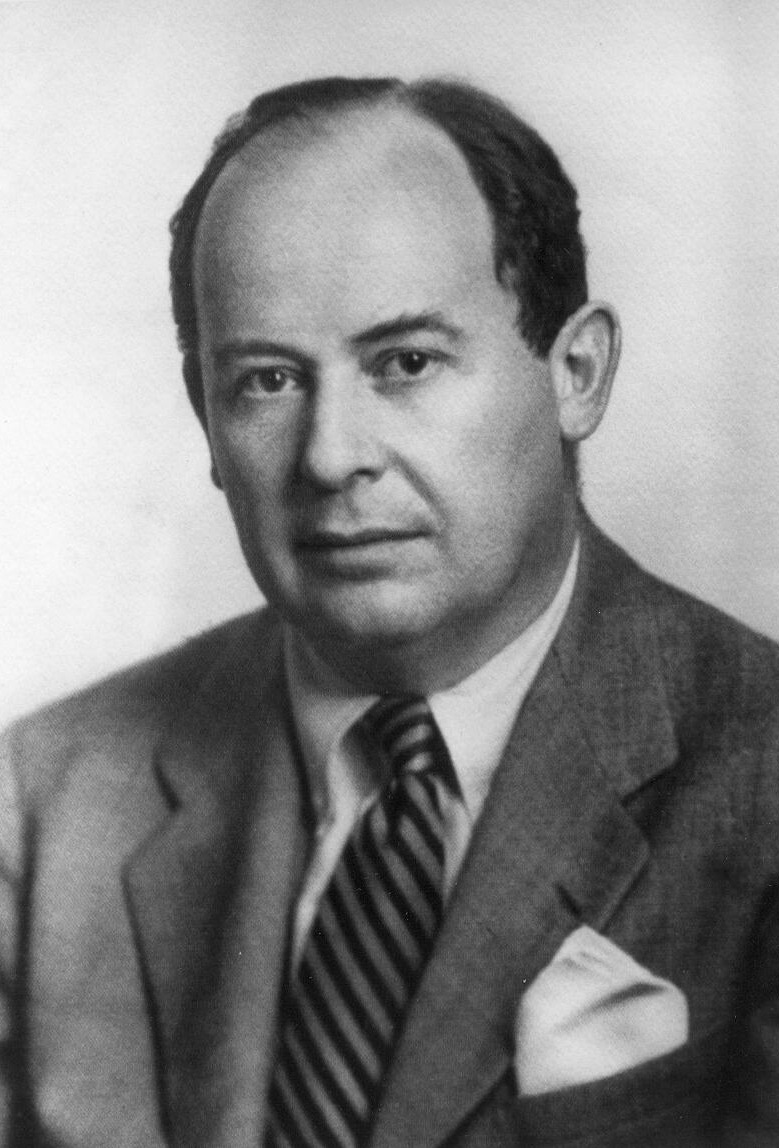
\includegraphics[width=\marginparwidth]{immagini/von_neu}
	\captionof{figure}[John von Neumann]{John von Neumann (Budapest, 28 dicembre 1903 --- Washington, 8 febbraio 1957).}
	\label{fig:vn}
%\end{figure}%
} struttura di un calcolatore descritta di seguito, attribuita al matematico e informatico \emph{John von Neumann} (figura~\ref{fig:vn} a lato), è rimasta pressoché immutata nel corso del tempo, sin dagli anni '40.
\begin{figure}
	\centering
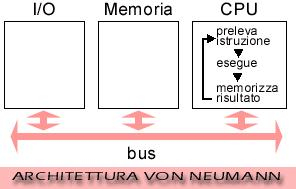
\includegraphics[width=0.45\columnwidth]{immagini/von_neumann}
	\caption[Calcolatore di von Neumann]{Struttura generale di un calcolatore di von Neumann.}
	\label{fig:neu}
\end{figure}
Il calcolatore, come schematizzato in figura~\ref{fig:neu}, è essenzialmente composto da:
\begin{description}
	\item
[\ac{cpu}] Nella \ac{cpu} (ovvero \emph{Unità Centrale d'Elaborazione}) vengono  trasformati e manipolati i dati;
	\item
[\ac{ram}] La \ac{ram} (ossia la \emph{Memoria di Lavoro}) è una memoria volatile: nel caso di spegnimento del computer, i dati contenuti in essa vanno perduti.
Serve per conservare i dati durante l'esecuzione di un programma (o l'elaborazione degli stessi);
	\item
[\ac{io}] Le unità di \ac{io}, cioè d'\emph{Ingresso/Uscita} consentono di immettere/acquisire dati nel/dal calcolatore e sono, ad esempio, tastiera (input), mouse (input), monitor (output), stampante (output), etc\dots
	\item
[Memoria Permanente] ossia quei supporti che conservano i dati a lungo termine, anche dopo lo spegnimento del calcolatore. Sono, ad esempio, dischi fissi, floppy, Compact Disc, etc\dots
\end{description}
Le prime tre componenti elencate sono assolutamente \emph{necessarie} ai fini del funzionamento del calcolatore e comunicano tra loro per mezzo del \emph{bus}\index{bus}.
Affinché le varie parti lavorino in modo sincrono, inoltre, in ogni macchina è presente il \emph{clock}\index{clock}, un apparecchio simile ad un metronomo che manda dei segnali ad ogni parte del computer e stabilisce la frequenza di lavoro.



La \ac{cpu} contiene dei registri adibiti alla conservazione di dati che è in grado di leggere ed utilizzare.
La \ac{ram}, in modo analogo, è organizzata in $n$ celle indicizzate da numeri interi non negativi e progressivi che partono da \num{0} e arrivano a $n-1$.
Affinché i programmi vengano eseguiti è necessario immettere nella memoria di lavoro le informazioni che sono composte, in genere, sia dai dati da elaborare che dalle istruzioni tramite cui avverrà l'elaborazione.

La \marginpar{Funzionamento della \ac{cpu}} macchina (o meglio, più strettamente parlando, la \ac{cpu}) per funzionare esegue tre operazioni principali:
\begin{description}[]
	\item
[Fetch\index{fetch}] Reperisce nella memoria di lavoro la prossima istruzione da eseguire.
Tra i registri della \ac{cpu}, infatti, ve n'è uno dedicato a contenere il numero della cella (chiamato anche \emph{indirizzo}\index{indirizzo}) della \ac{ram} contenente l'istruzione successiva;
	\item
[Decode\index{decode}] Una volta trovata l'istruzione da eseguire è necessario che questa venga decodificata dalla \ac{cpu};
	\item
[Execute\index{execute}] Avvenuta la decodifica, la \ac{cpu} esegue l'istruzione.
In generale, ciò comporta una modifica del contenuto dei registri: in particolare, cambierà almeno il contenuto del \emph{program counter}\index{program counter} (il registro della \ac{cpu} che contiene l'indirizzo dell'istruzione successiva).
\end{description}

	\section{Rappresentazione della memoria del calcolatore e tipi di dato semplici}
	\label{sec:mem}
Può tornare utile immaginare la memoria di un computer come un foglio a quadretti che rappresentano le celle della \ac{ram}.\footnote{Per gli attuali calcolatori, anche quelli presenti in ambienti domestici, il numero di ``quadretti'' è dell'ordine di \num{e9}.}
Ogni quadretto può contenere uno ed un solo ``dato semplice'' come,  ad esempio, un carattere, un numero, o qualsiasi altro \emph{simbolo}.

Ogni dato, di qualsiasi tipo, occupa una certa quantità di celle, ciascuna delle quali è identificata da un numero progressivo: il suddetto \emph{indirizzo}. %\footnote{Il calcolatore non è in grado di ``comprendere'' la numerazione decimale. Esso è in grado di codificare solo istruzioni che gli vengano passate in linguaggio binario.}
Spesso è abbastanza scomodo usare gli indirizzi per individuare la posizione dei dati, pertanto possiamo contrassegnare uno o più quadretti consecutivi con un nome simbolico.
In\marginpar{Variabili} questo modo identifichiamo dei blocchi di quadretti  chiamati \emph{variabili}\index{variabile}.


Le variabili vengono classificate in \emph{tipi}\marginpar{Tipi}\index{tipo}.
Il concetto di tipo non è una caratteristica di tutti i linguaggi di programmazione: in \lang{C} è \emph{necessario} specificare il tipo di una variabile ma lo stesso non vale, ad esempio, per linguaggi come il \lang{Python}.
Ad ogni tipo di dato corrisponde una particolare quantità di memoria che il calcolatore \emph{alloca} (alcuni tipi richiedono più celle di altri).
I \emph{tipi primitivi}\index{tipo!primitivo} in linguaggio \lang{C} sono:
\begin{description}
	\item\lstinline!char! Indica un carattere (lettera , cifra, segno\dots) ed occupa \emph{una} cella;
	\item\lstinline!int! Indica un numero intero (anche negativo, cioè appartenente a $\mathbb{Z}$);
	\item\lstinline!float! Indica un numero decimale.
Questa dovrebbe essere la rappresentazione di un numero reale all'interno del calcolatore tuttavia non ci è possibile memorizzare un numero con infinite cifre dopo la virgola.
Pertanto questo tipo è solo una rappresentazione approssimata di un numero irrazionale (o razionale periodico).
\end{description}

	\section{Programmazione imperativa ed assegnamenti}
Esistono diversi \emph{paradigmi}\index{paradigma} (schemi generali) di programmazione.
Qui ci occuperemo della \emph{programmazione imperativa} in cui l'operazione principale è l'\emph{assegnamento}\index{assegnamento}\marginpar{Assegnamento}, definito come il processo di inserimento dei dati nelle celle.
La sintassi per un assegnamento in \lang{C} è 
\begin{lstlisting}
£!\MyComment{nome}!£ = £!\MyComment{valore}!£;
\end{lstlisting}
Si noti che ogni istruzione \emph{deve} terminare con il punto e virgola (che d'ora in poi verrà spesso omesso per motivi tipografici) come, ad esempio la scrittura
\begin{lstlisting}
variabile = 5303;
\end{lstlisting}
Un'istruzione d'assegnamento è formata da tre parti:
\begin{itemize}
	\item
Il \MyComment{nome} della variabile, in questo caso ``\lstinline!variabile!'';
	\item
Operatore di assegnamento ``\lstinline!=!'', da non confondere con l'operatore relazionale ``\lstinline!==!'';
	\item
Il \MyComment{valore} della variabile, ad esempio \num{5303}, che deve essere \emph{compatibile} con il suo tipo.\footnote{%Le variabili di tipo \lstinline!float! contengono un numero decimale; 
%Si tenga presente che un assegnamento per una variabile di questo tipo dev'essere, ad esempio, \lstinline!f = 23.934;!.
La virgola per gli assegnamenti a variabili \lstinline!float! è di tipo \emph{anglosassone}: il compilatore non riconoscerà un numero del tipo \lstinline!f = 23,934!.
}
\end{itemize}
Sono ammessi assegnamenti anche del tipo
\begin{lstlisting}
variabile2 = variabile;
\end{lstlisting}
a patto che le \lstinline!variabile! e \lstinline!variabile2! abbiano dei tipi compatibili tra di loro.
Con questo assegnamento, anche la variabile \lstinline!variabile2! ora ha il valore \num{5303}.


Gli assegnamenti possono contenere anche delle funzioni (matematiche) come, ad esempio
\begin{lstlisting}
y = v / 10;
\end{lstlisting}
Se \lstinline!v! è di tipo \lstinline!int!, supponiamo che valga \num{58}, il risultato della divisione (e quindi il valore di \lstinline!y!) sarà un ancora un intero, cioè \num{5}.
Se, invece, \lstinline!v! è di tipo \lstinline!float!, otterremo come risultato \num{5.8}.


Esistono degli assegnamenti in cui la stessa variabile compare da entrambe le parti come, ad esempio
\begin{lstlisting}
x = x + 1;
\end{lstlisting}
Questa istruzione legge il valore di \lstinline!x!, calcola il risultato della somma e lo ri-assegna a \lstinline!x!.
Supponiamo ora di avere una variabile \lstinline!float beta! con un certo valore che noi vogliamo triplicare.
Si può usare l'istruzione
\begin{lstlisting}
beta = 3 * beta;
\end{lstlisting}
Malgrado \num{3} non sia di tipo \lstinline!float!, il risultato del prodotto (cioè \num{30.9}) lo sarà.


Per \marginpar{Dichiarazione} comunicare al computer il tipo di variabile che intendiamo usare, dobbiamo effettuare la già citata operazione di \emph{dichiarazione}\index{dichiarazione}.
In \lang{C}, essa assume la forma ``\lstinline!float gamma;!'', oppure:
\begin{lstlisting}
float beta, gamma;
gamma = 1.0;
beta = gamma + 5;
\end{lstlisting}
In generale, tutte le dichiarazioni vanno poste all'inizio del programma

Il \lang{C} dispone anche di operatori aritmetici. I \marginpar{Principali operatori algebrici} principali operatori sono: \lstinline!+! (operatore somma), \lstinline!-! (operatore differenza), \lstinline!*! (operatore prodotto), \lstinline!/! (operatore quoziente), \lstinline!%! (operatore modulo, restituisce il resto di una divisione). Ad esempio:
\begin{lstlisting}
int z;
z = 5 % 3;
\end{lstlisting}
restituisce un valore \lstinline!z = 2!.

	\section{Strutture di controllo}
	\label{sec:ContStruc}
L'ordine con cui vengono eseguite le istruzioni dipende dalle \emph{strutture di controllo}.
Esse sono, essenzialmente, gli assegnamenti ed altre poche istruzioni ed hanno il compito di ``gestire'' e, appunto, controllare il flusso delle informazioni durante l'esecuzione di un programma.
Qualunque algoritmo può essere espresso per mezzo di tre strutture di controllo:
\begin{itemize}
	\item
Sequenza;
	\item
Scelta;
	\item
Iterazione.
\end{itemize}

		\subsection{Sequenza}

La \emph{sequenza} è determinata dall'ordine in cui vengono scritte le istruzioni nel codice sorgente.
Per convenzione la ``lettura'' avviene dall'alto in basso e da sinistra verso destra così istruzioni scritte ``in alto'' verranno eseguite prima di istruzioni scritte ``in basso''.

		\subsection{Scelta}
In linguaggio \lang{C}, la scelta si riconosce dalla preposizione \lstinline!if!, come nel codice

\begin{lstlisting}
if ( x < 0 )
	x = -x;
\end{lstlisting}
Le parentesi tonde racchiudono la \emph{condizione}\index{condizione}, talvolta chiamata \emph{test}\index{test}, che deve essere verificata affinché il corpo della scelta venga eseguito e sono sintatticamente obbligatorie.
Se la condizione non è verificata, il corpo della scelta (in questo caso rappresentato dall'unica istruzione ``\lstinline!x = -x!'') non viene eseguito.
\`E possibile che il corpo sia composto da più di un'istruzione, come nel codice~\ref{code:corpo} nel riquadro~\ref{riq:IfChoose}, nel qual caso le istruzioni vanno incluse tra parentesi graffe e formano un \emph{blocco}\index{blocco}.
%Se ne vedranno degli esempi in seguito.

\begin{table}
\centering
	\caption{Alcuni operatori nel linguaggio \lang{C}.}
	\label{tab:op}
\subfloat[][Operatori logici.\label{tab:lop}]{
\begin{tabular}{>$l<$ F >$l<$ F}
		\toprule
\text{Condizione} &$\textrm{Operatore}$  &\textrm{Esempio\dots} &$\textrm{\dots{}in \lang{C}}$\\
		\midrule
C_1\land C_2	&\&\&		&a< x< b			&x > a  \&\& x < b\\
C_1\lor C_2	&||			&x<a\lor x>b 		&x < a \|\| x > b\\
\text{Non }C_1	&{!}			&x \neq b			&!(  x = b )\\
		\bottomrule
	\end{tabular}
}\\
\subfloat[][Operatori relazionali.\label{tab:lop}]{
\begin{tabular}{FF}
\toprule
$\text{Operatore}$ &{a} \\
\midrule
<	&\\
<=	&\\
>	&\\
>=	&\\
==	&\\
!=	&\\
\bottomrule
\end{tabular}
}
\end{table}
Nel test si possono usare gli operatori logici e relazionali elencati nella tabella~\ref{tab:op}.

%Per \marginpar{Operatori relazionali} il test, si dispone dei seguenti operatori relazionali: \lstinline!<! (operatore minore), \lstinline!<=! (operatore minore o uguale), \lstinline!>! (operatore maggiore), \lstinline!>=! (operatore maggiore o uguale), \lstinline!==! (operatore uguale), \lstinline?!=? (operatore diverso\footnote{In generale, il simbolo \lstinline?!? nei test equivale ad una negazione. Quindi \lstinline?!=? starebbe a significare ``non uguale'', cioè diverso.}).


\begin{code}
\begin{minipage}{0.45\columnwidth}
	\begin{lstlisting}[caption={\ },nolol]
if ( x < 0 )
	x = - x;
else
	x = x + 3;
	\end{lstlisting}
\end{minipage}	\hfill
\begin{minipage}{0.45\columnwidth}
	\begin{lstlisting}[caption={\ },nolol]
if ( x < 0 )
	x = - x;
else
	x = x + 3;
	\end{lstlisting}
\end{minipage}	\hfill
\begin{minipage}{0.45\columnwidth}
	\begin{lstlisting}[caption={\ },nolol,label={code:corpo}]
if ( x < 0 ) {
	x = - x;
	y = 3 + z;
	e = y + 1;
}
else
	£!\MyComment{\dots}!£
	\end{lstlisting}
\end{minipage}	\hfill
\begin{minipage}{0.45\columnwidth}
\begin{lstlisting}[caption={\ },nolol]
if ( £!\MyComment{test\_1}!£ )
	if ( £!\MyComment{test\_2}!£ )
		£!\MyComment{\dots}!£
	else
		£!\MyComment{\dots}!£
else
	£!\MyComment{\dots}!£
	\end{lstlisting}
\end{minipage}	\hfill
\begin{minipage}{0.45\columnwidth}
	\begin{lstlisting}[caption={\ },nolol]
if ( £!\MyComment{test\_1}!£ ) 
	£!\MyComment{\dots}!£
else
	if ( £!\MyComment{test\_2}!£  )
		£!\MyComment{\dots}!£
	else
		£!\MyComment{\dots}!£
	\end{lstlisting}
\end{minipage}	\hfill
\begin{minipage}{0.45\columnwidth}
	\begin{lstlisting}[caption={\ },nolol]
if (  £!\MyComment{test\_1}!£ ) 
	£!\MyComment{\dots}!£
else if ( £!\MyComment{test\_2}!£ )
		£!\MyComment{\dots}!£
	else
		£!\MyComment{\dots}!£
	\end{lstlisting}
\end{minipage}
\caption{Sintassi della scelta \lstinline!if!.}
\label{riq:IfChoose}
\end{code}
È possibile trovare anche scelte che presentano le sintassi elencate nel riquadro~\ref{riq:IfChoose}.
Nel codice~\ref{code:corpo}, il corpo della scelta \lstinline!if! è composto da tutte le istruzioni contenute tra parentesi graffe.
Il calcolatore le esegue come se fossero una sola istruzione (naturalmente, rispettando la convenzione di eseguire prima quelle scritte  in alto).

\begin{lstlisting}[
	caption={[Struttura di un programma in linguaggio \lang{C}.] {Struttura generale di un programma in linguaggio \lang{C}.}},%
	float,%
	label={cod:GenProSyn}%
]
#include <stdio.h>

int main ( void ) {
	int x, y;
	float z, f;

	£!\MyComment{istruzioni}!£

	exit( £!\MyComment{valore}!£ );
}
\end{lstlisting}
In \marginpar{Struttura caratteristica di un programma in \lang{C}} generale, un programma scritto in \lang{C} ha una struttura generale caratteristica. Essa si ripresenta quasi uguale nella maggior parte dei programmi ed è mostrata nel codice~\ref{cod:GenProSyn}.
